\begin{figure}

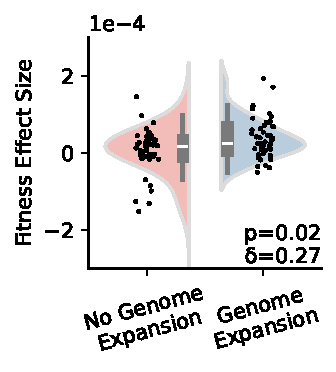
\includegraphics[width=0.52\linewidth]{%
binder-2025-09-05-genome-expansion-fitness/binder/teeplots/2025-09-05-genome-expansion-fitness/biotic_background=Contemporary(no diversity maint.)+hue=genome-expansion+palette=pastel1+subject=Specimen+test=mw+viz=violinplot+x=genome-expansion+y=fitness-differential-focal+ext=.pdf}
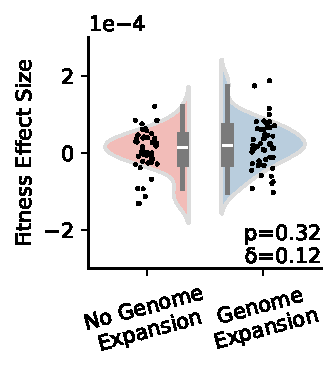
\includegraphics[width=0.405\linewidth, trim={1.3cm 0 0 0.6cm}, clip]{%
binder-2025-09-05-genome-expansion-fitness/binder/teeplots/2025-09-05-genome-expansion-fitness/biotic_background=Prefatory(no diversity maint.)+hue=genome-expansion+palette=pastel1+subject=Specimen+test=mw+viz=violinplot+x=genome-expansion+y=fitness-differential-focal+ext=.pdf}%

\vspace{-1ex}

\begin{subfigure}{0.135\linewidth}
~
\end{subfigure}%
\begin{subfigure}{0.405\linewidth}
    \centering
    \caption{\footnotesize contemporary\\background\\(no diversity maint.)}
    \label{fig:genome-expansion-nodmaint:contemporary}
\end{subfigure}%
\begin{subfigure}{0.405\linewidth}
    \centering
    \caption{\footnotesize prefatory\\background\\(no diversity maint.)}
    \label{fig:genome-expansion-nodmaint:prefatory}
\end{subfigure}%

\caption{
    \textbf{Co-occurence of adaptation with genome expansion, specimen assays without diversity maintenance.}
    \footnotesize
    Violin plots compare adaptation assay outcome distributions between focal specimens with genome size increase relative to ancestor and those without.
    Assays compete focal specimen at stint $n+1$ against focal population at stint $n$;
    panels report outcomes under two assay designs, differing in biotic context.
    When competed in the presence of background strain population from stint $n+1$, stronger adaptation accompanies genome expansions --- with small effect size (panel \ref{fig:genome-expansion-nodmaint:contemporary}; $p = 0.02, \; \delta = 0.27$).
    By contrast, no effect is apparent under prefatory biotic background from stint $n$ (panel \ref{fig:genome-expansion-nodmaint:prefatory}).
    Reported statistics are Cliff's delta, a non-parametric effect size metric ranging from 0.0 to 1.0, and two-tailed Mann-Whitney U test.
    Results are consistent with assays conducted with balancing procedures for diversity maintenance with background strain enabled, reported in Figure \ref{fig:genome-expansion}.
}
\label{fig:genome-expansion-nodmaint}

\end{figure}
